% Required packages: \usepackage{amsmath}, \usepackage{graphicx}, \usepackage{multirow}
\begin{table}[h!]
\centering
\renewcommand{\arraystretch}{1.4}
\resizebox{\textwidth}{!}{%
\begin{tabular}{lccccccccc}
\toprule
\multirow{2}{*}{\textbf{Célula}} & \textbf{$k$} & \textbf{$a$} & \textbf{$b$} & \textbf{$d$} & \textbf{$C_m$} & \textbf{$V_r$} & \textbf{$V_t$} & \textbf{$V_{min}$} & \textbf{$V_{peak}$} \\
 & (nS/mV) & (ms$^{-1}$) & (nS) & (pA) & (pF) & (mV) & (mV) & (mV) & (mV) \\
\midrule
$\vcenter{\hbox{
\includegraphics[height=1.5em]{figuras/neurônios/mgc.png}}}$ Granular madura & 0.45 & 0.003 & 24.48 & 50 & 38 & -77.4 & -44.9 & -66.47 & 15.49 \\
$\vcenter{\hbox{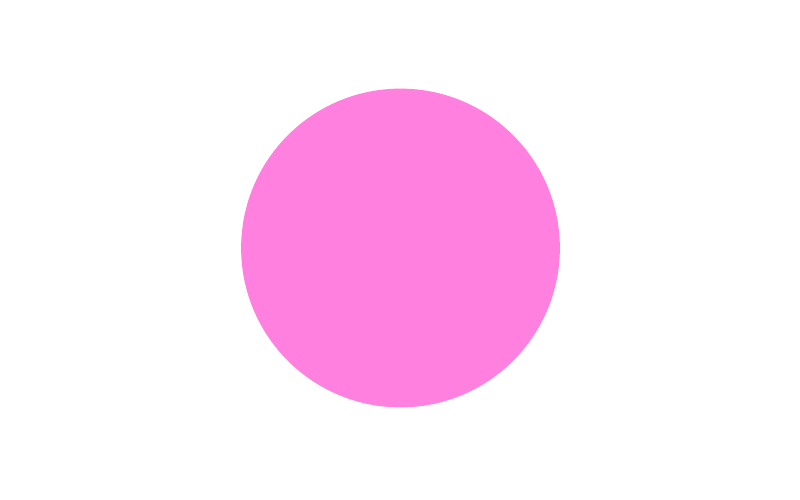
\includegraphics[height=1.5em]{figuras/neurônios/igc.png}}}$ Granular imatura & 0.139 & 0.002 & -1.877 & 12.149 & 24.6 & -63.66 & -38.41 & -48.2 & 83.5 \\
$\vcenter{\hbox{
\includegraphics[height=1.5em]{figuras/neurônios/mc.png}}}$ Musgosa & 1.5 & 0.004 & -20.84 & 117 & 258 & -63.67 & -37.11 & -47.98 & 28.29 \\
$\vcenter{\hbox{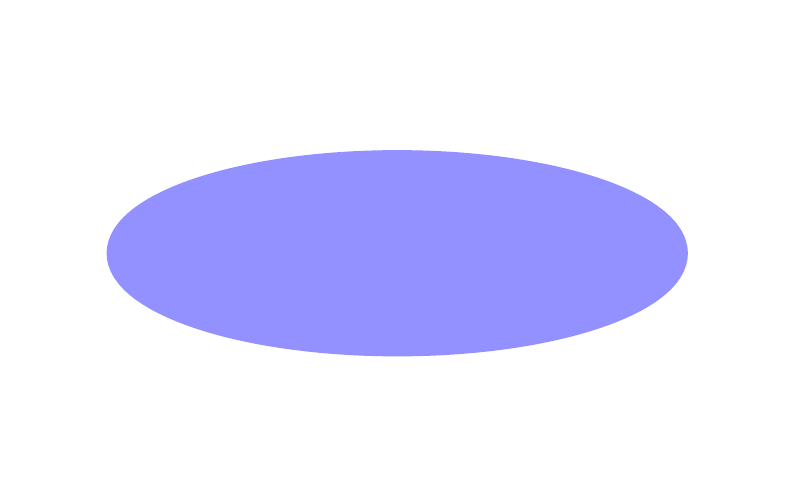
\includegraphics[height=1.5em]{figuras/neurônios/hipp.png}}}$ HIPP & 0.01 & 0.004 & -2 & 40.52 & 58.7 & -70 & -50 & -75 & 90 \\
$\vcenter{\hbox{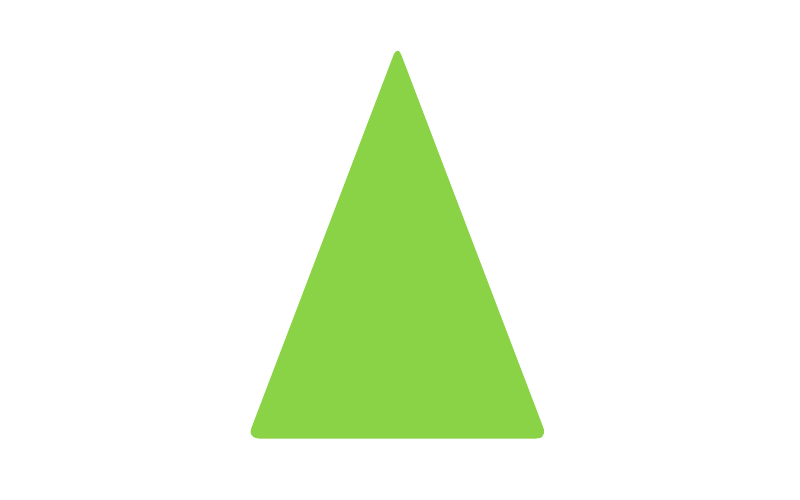
\includegraphics[height=1.5em]{figuras/neurônios/bc.png}}}$ Em cesto & 0.81 & 0.097 & 1.89 & 553 & 208 & -61.02 & -37.84 & -36.23 & 14.08 \\
$\vcenter{\hbox{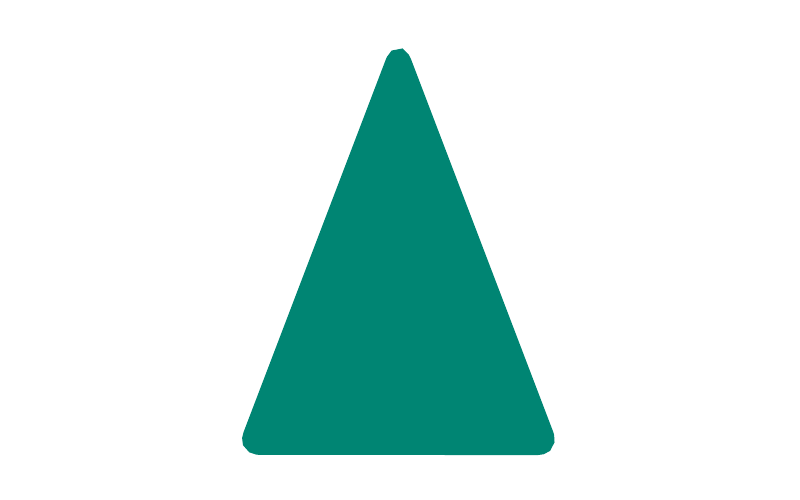
\includegraphics[height=1.5em]{figuras/neurônios/pca3.png}}}$ Piramidal do CA3 & 0.79 & 0.008 & -42.55 & 588 & 366 & -63.2 & -33.6 & -38.87 & 35.86 \\
$\vcenter{\hbox{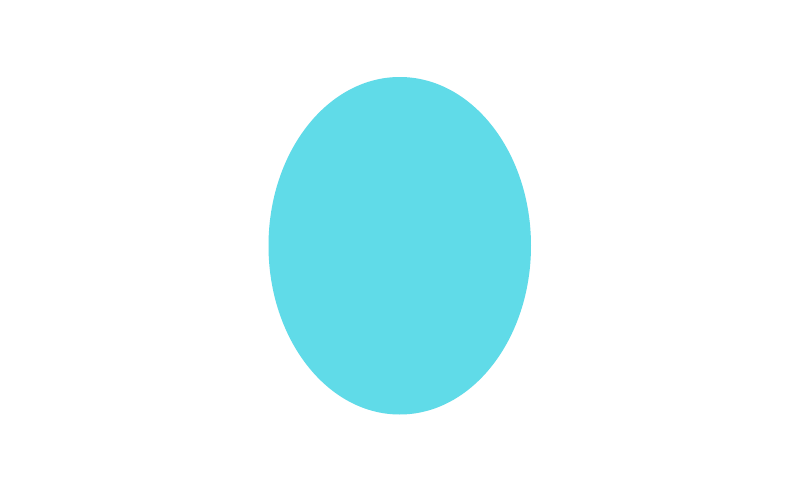
\includegraphics[height=1.5em]{figuras/neurônios/ica3.png}}}$ Inibitória do CA3 & 1 & 0.004 & 9.26 & -6 & 45 & -57.51 & -23.38 & -47.56 & 18.45 \\
\bottomrule
\end{tabular}}
\caption{Parâmetros do modelo Izhikevich por tipo de neurônio.}\label{tab:izhikevich_neuron_params}
\end{table}
